\chapter{Aufbau eines Prototypen}
\section{H-Brücke}
Die Brückenschaltung orientiert sich an der Schaltung des zuvor verwendeten Motortreibers sowie an der vorgeschlagenen Schaltung aus dem Datenblatt der Halbbrücken und erlaubt, dass sich der Motor je nach Durchschalten in beide Richtungen drehen kann.
Als Halbbrücken dienen zwei BTN8982 mit jeweils einem p-channel highside MOSFET und einem n-channel lowside MOSFET mit bereits integrierten Schutzmechanismen wie Abschaltung bei zu geringer Spannung oder Übertemperatur beinhalten.  Das Blockdiagramm dieser Halbbrücken ist in nachstehender Abbildung dargestellt.
\begin{figure}[h]
	\centering
		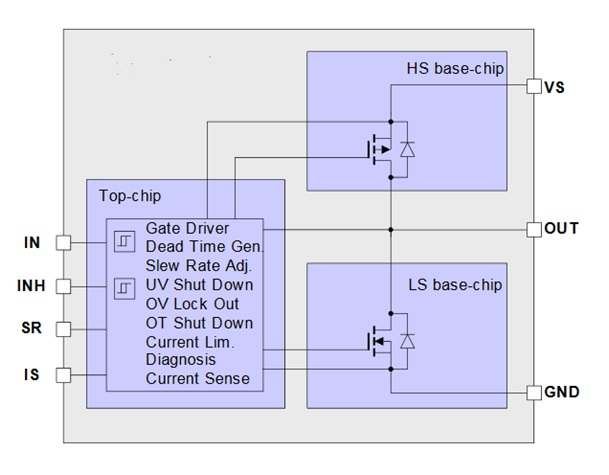
\includegraphics{Bilder/Blockdiagramm Halbbruecken.jpg}
	\caption{Blockdiagramm Halbbrücken}
	\label{fig:Blockdiagramm Halbbruecken}
\end{figure}
In dem Blockdiagramm sind bereits die PINs der Halbbrücken zu erkennen. Diese sollen nun in Tabelle \ref{tab:Pinverteilung} nochmal aufgezählt und ihre Funktionen erklärt werden.

\begin{table}[h]
	\centering
		\begin{tabular}{l|p{7cm}|p{7cm}}
			Pin Nummer & Bezeichnung & Erläuterung & Anschluss an \\ \hline
		\end{tabular}
	\caption{Pinverteilung Halbbrücken}
	\label{tab:Pinverteilung}
\end{table}
